\documentclass[14 pt, fleqn]{extarticle}

	\usepackage[frenchb]{babel}
	\usepackage[utf8]{inputenc}  
	\usepackage[T1]{fontenc}
	\usepackage{amssymb}
	\usepackage[mathscr]{euscript}
	\usepackage{stmaryrd}
	\usepackage{amsmath}
	\usepackage{tikz}
	\usepackage[all,cmtip]{xy}
	\usepackage{amsthm}
	\usepackage{varioref}
	\usepackage{geometry}
	\geometry{a4paper}
	\usepackage{lmodern}
	\usepackage{hyperref}
	\usepackage{array}
	 \usepackage{fancyhdr}
	 \usepackage{float}\usepackage{setspace}
\setlength{\mathindent}{1cm}
\renewcommand{\theenumi}{\alph{enumi})}
	\pagestyle{fancy}
	\theoremstyle{plain}
	\fancyfoot[C]{} 
	\fancyhead[L]{}
	\fancyhead[R]{}\geometry{
 a4paper,
 total={170mm,257mm},
 left=5mm,
 top=5mm,
 bottom = 0mm
 }
	
	
	\title{Exercices de calcul}
	\date{}
	\begin{document}
	 
\subsection*{Exercice 1 - Fonction donnée par un programme de calcul}	 
	 
	 On considère le programme de calcul suivant : 
	 \begin{itemize}
	 \item Choisir un nombre.
	 \item Le mettre au carré 
	 \item Lui ajouter 3 
	 \item Diviser par 2.
	 \end{itemize}
	 
	 \begin{enumerate}
	 \item Que donne le programme lorsqu'on choisit le nombre $2$ ? 
	 \item On note $f(x)$ le nombre obtenu quand on choisit le nombre $x$. Donnez une expression de $f(x)$ en fonction de $x$. 
	 \item Donnez l'image de $-5$ par $f$. 
	 \item Donnez un antécédent de $4$ par $f$.Combien y en a-t-il ? 
	 \item Remplir le tableau suivant : 
	 
\begin{figure}[H]
\center
$\begin{array}{|c|c|c|c|c|c|}
\hline
 x &  2 & -5 & \frac12 &    &   \\
\hline
f(x)&   & & & 4 &   6   \\
\hline
\end{array}$
\end{figure}

	 \end{enumerate}
	 
	 
	 
\subsection*{Exercice 2 - Fonction donnée par un tableau de valeurs}	 
	 
On considère une fonction $g$ dont un tableau de valeurs est le suivant : \begin{figure}[H]
\center
$\begin{array}{|c|c|c|c|c|c|}
\hline
 x &  -2 & -1 & 3 & 6  &  2 \\
\hline
g(x)&  5 & -3  & 3 & 14 &   6   \\
\hline
\end{array}$
\end{figure}	 

\begin{enumerate}
\item Donnez une image de $6$ par $f$. 
\item Donnez un antécédent de $6$ par $f$. 
\item Donnez un nombre tel que $f(x)=x$.
\end{enumerate}


\subsection*{Exercice 3 - Fonction donnée par une expression algébrique}	 
	 
On considère une fonction $h$ définie par $h(x)= 5(x+4) -2$. 
\begin{enumerate}
\item Donnez un programme de calcul qui calcule le résultat de $h$. 
\item Développez et réduire l'expression de $h(x)$. 
\item Calculez l'image de $4$ par $h$. 
\item Donnez un antécédent de $33$ par $h$. 
\item Remplir le tableau suivant : 
	 
\begin{figure}[H]
\center
$\begin{array}{|c|c|c|c|c|c|}
\hline
 x &  2 & -5 & \frac12 &    &   \\
\hline
h(x)&   & & & 14 &   \frac34   \\
\hline
\end{array}$
\end{figure}
\end{enumerate} 

	 
\subsection*{Exercice 4 - Fonction donnée par une courbe}	 
	 
	 On considère la fonction $g$ dont la courbe représentative est sur le tableau suivant. 
\[ 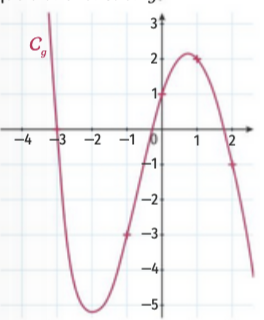
\includegraphics{Courbe1}	 \]
\begin{enumerate}
\item Remplir le tableau de valeurs suivant. 
	 \begin{figure}[H]
\center
$\begin{array}{|c|c|c|c|c|c|}
\hline
 x & -3  &  &  & 1 & 2 \\
\hline
h(x)&  & -3 & 1 &  &  \\
\hline
\end{array}$
\end{figure}

\item Combien existe-t-il d'antécédents de $1$ par $g$ ? 
\end{enumerate}


\subsection*{Exercice 5 - Brevet métropole 2023}	

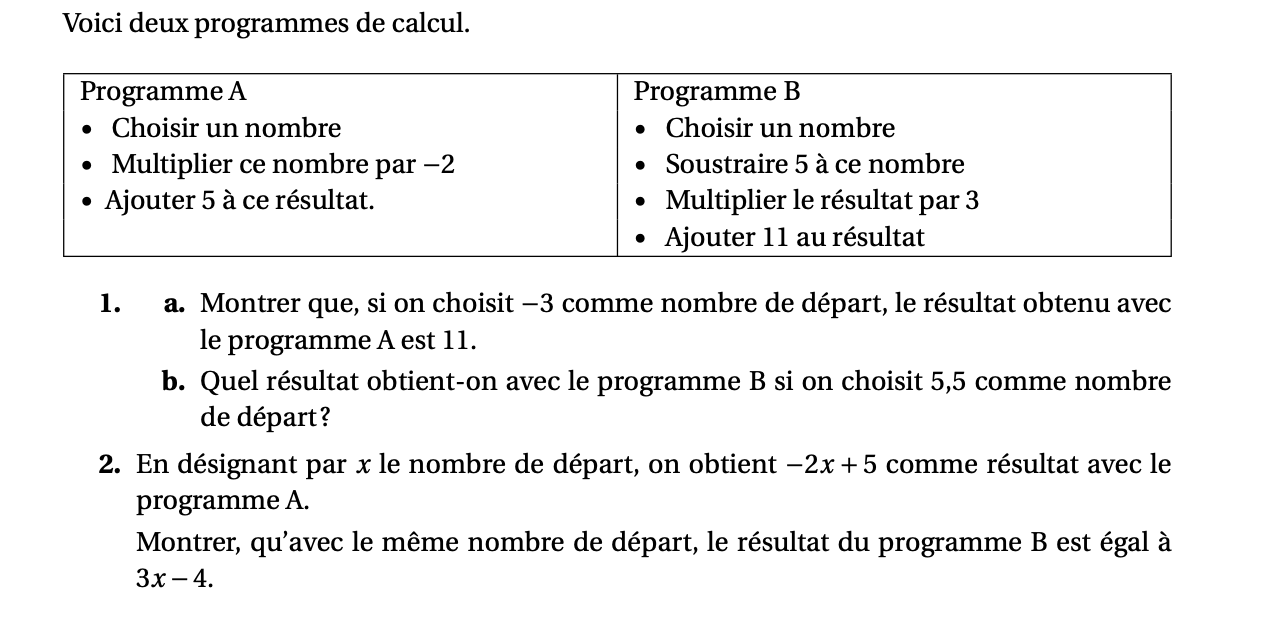
\includegraphics[width = 21 cm]{Ex51}
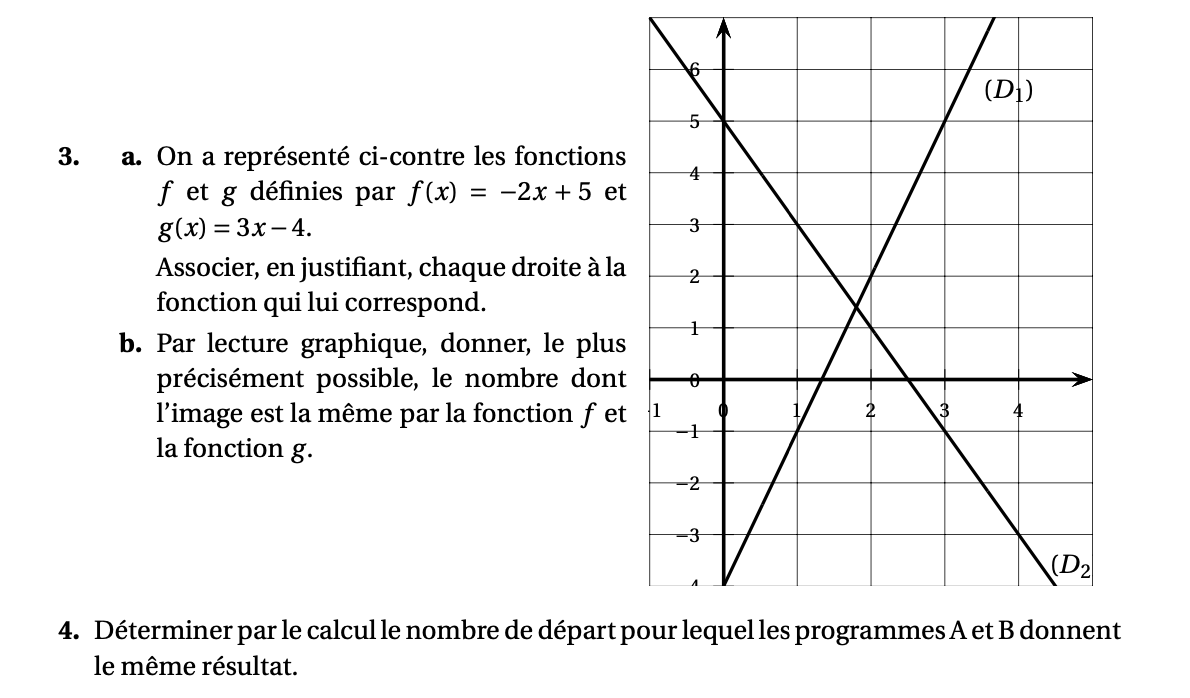
\includegraphics[width = 21 cm]{Ex52}


\subsection*{Exercice 6 - Polynésie 2022}	

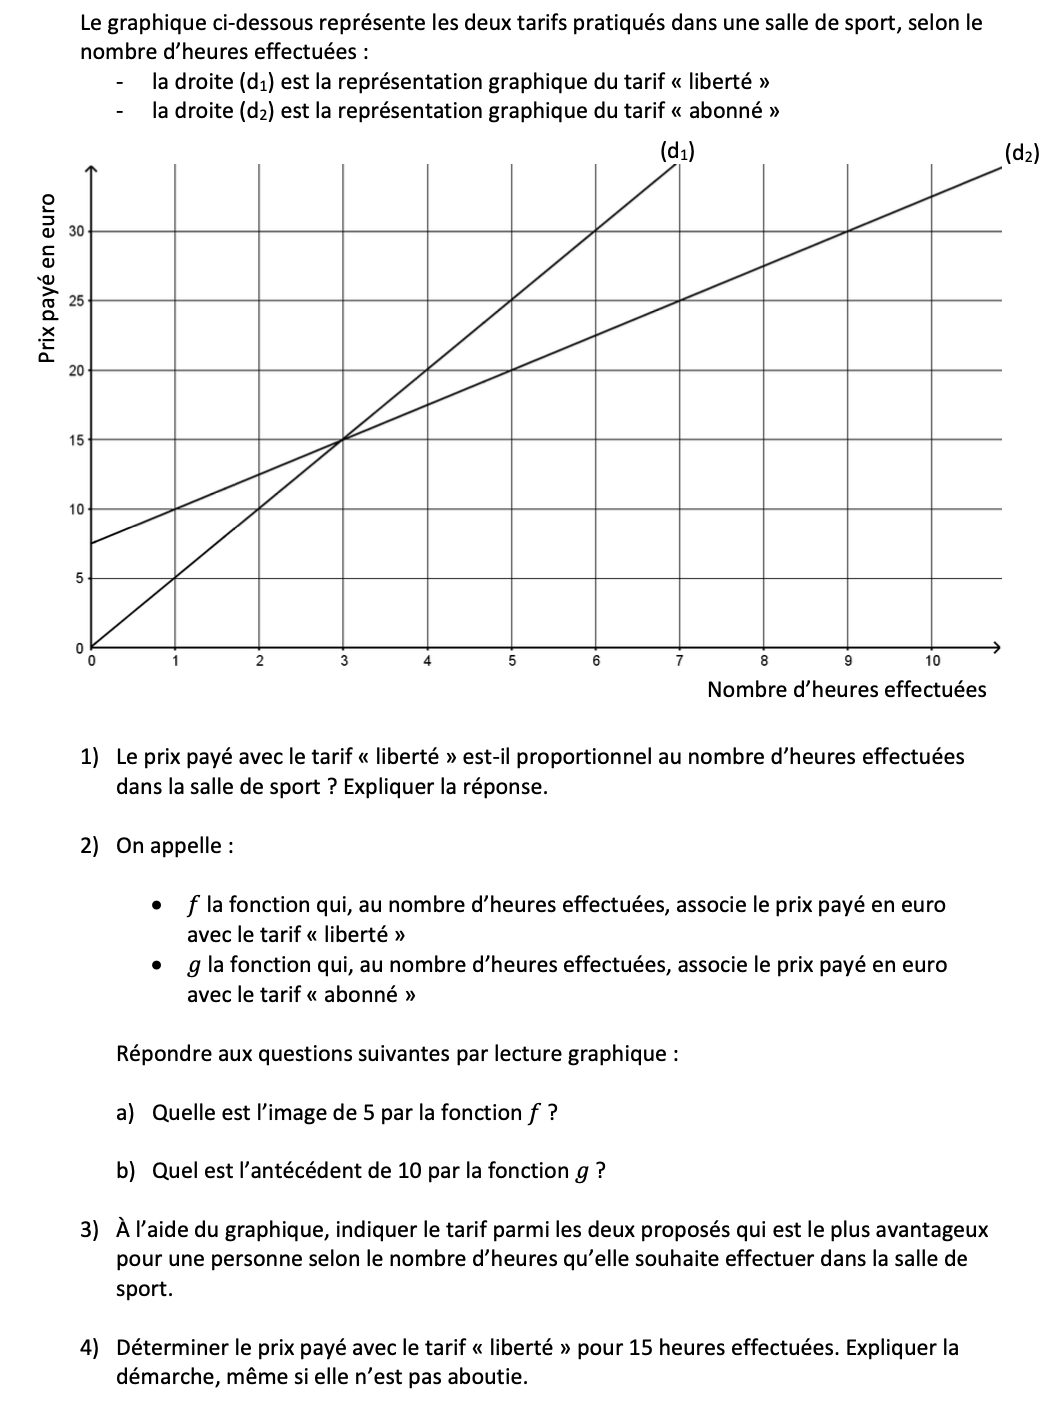
\includegraphics[width = 20 cm]{Ex6}


\subsection*{Exercice 7 - Nouvelle-Calédonie 2022}	

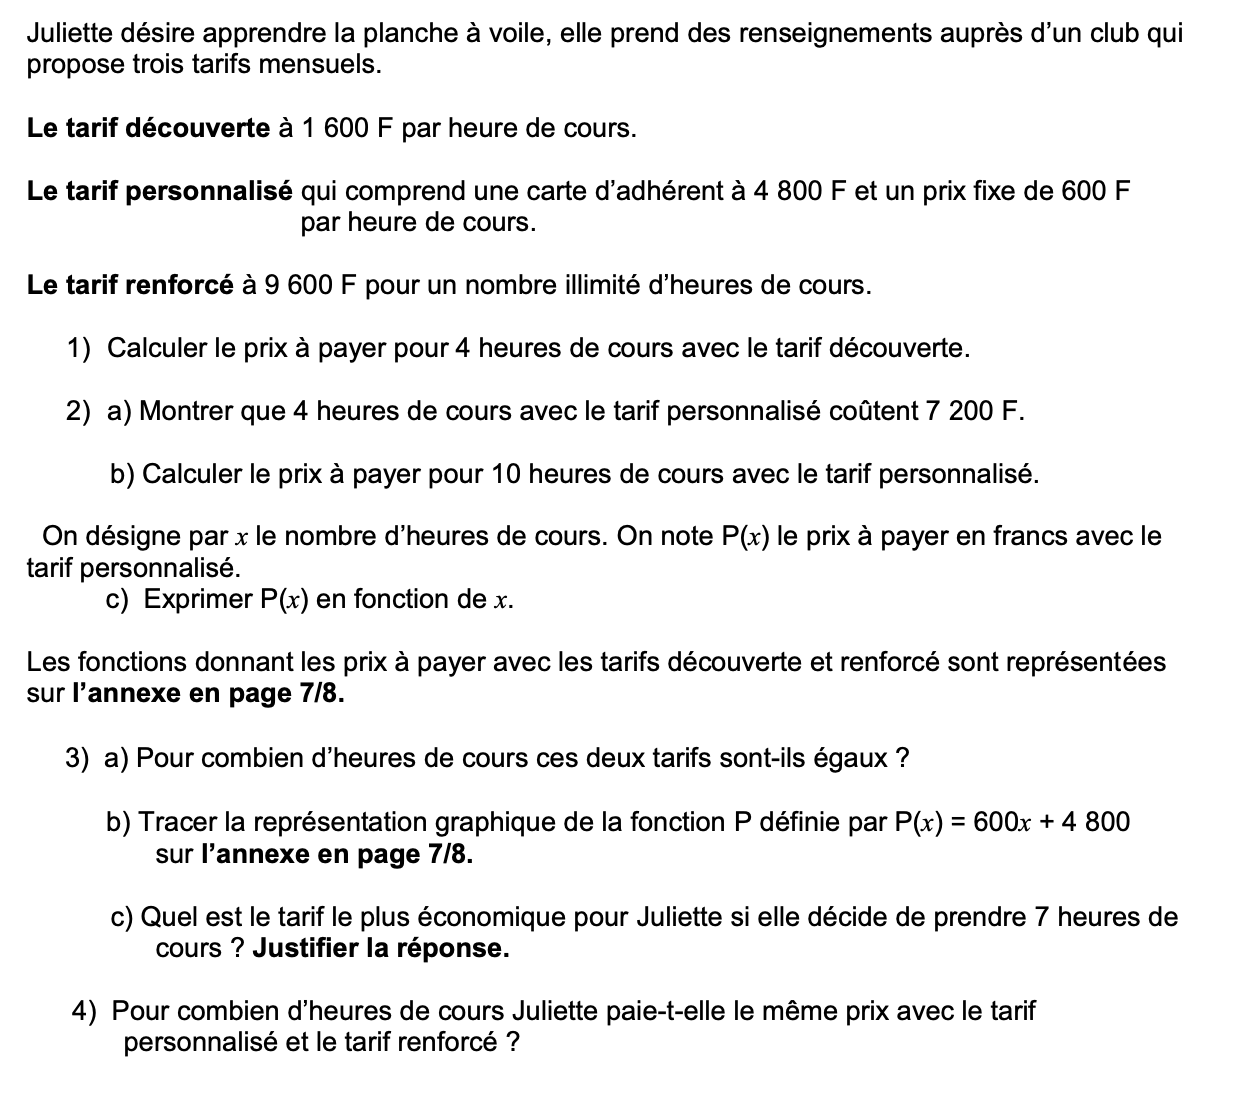
\includegraphics[width = 20 cm]{Ex7}
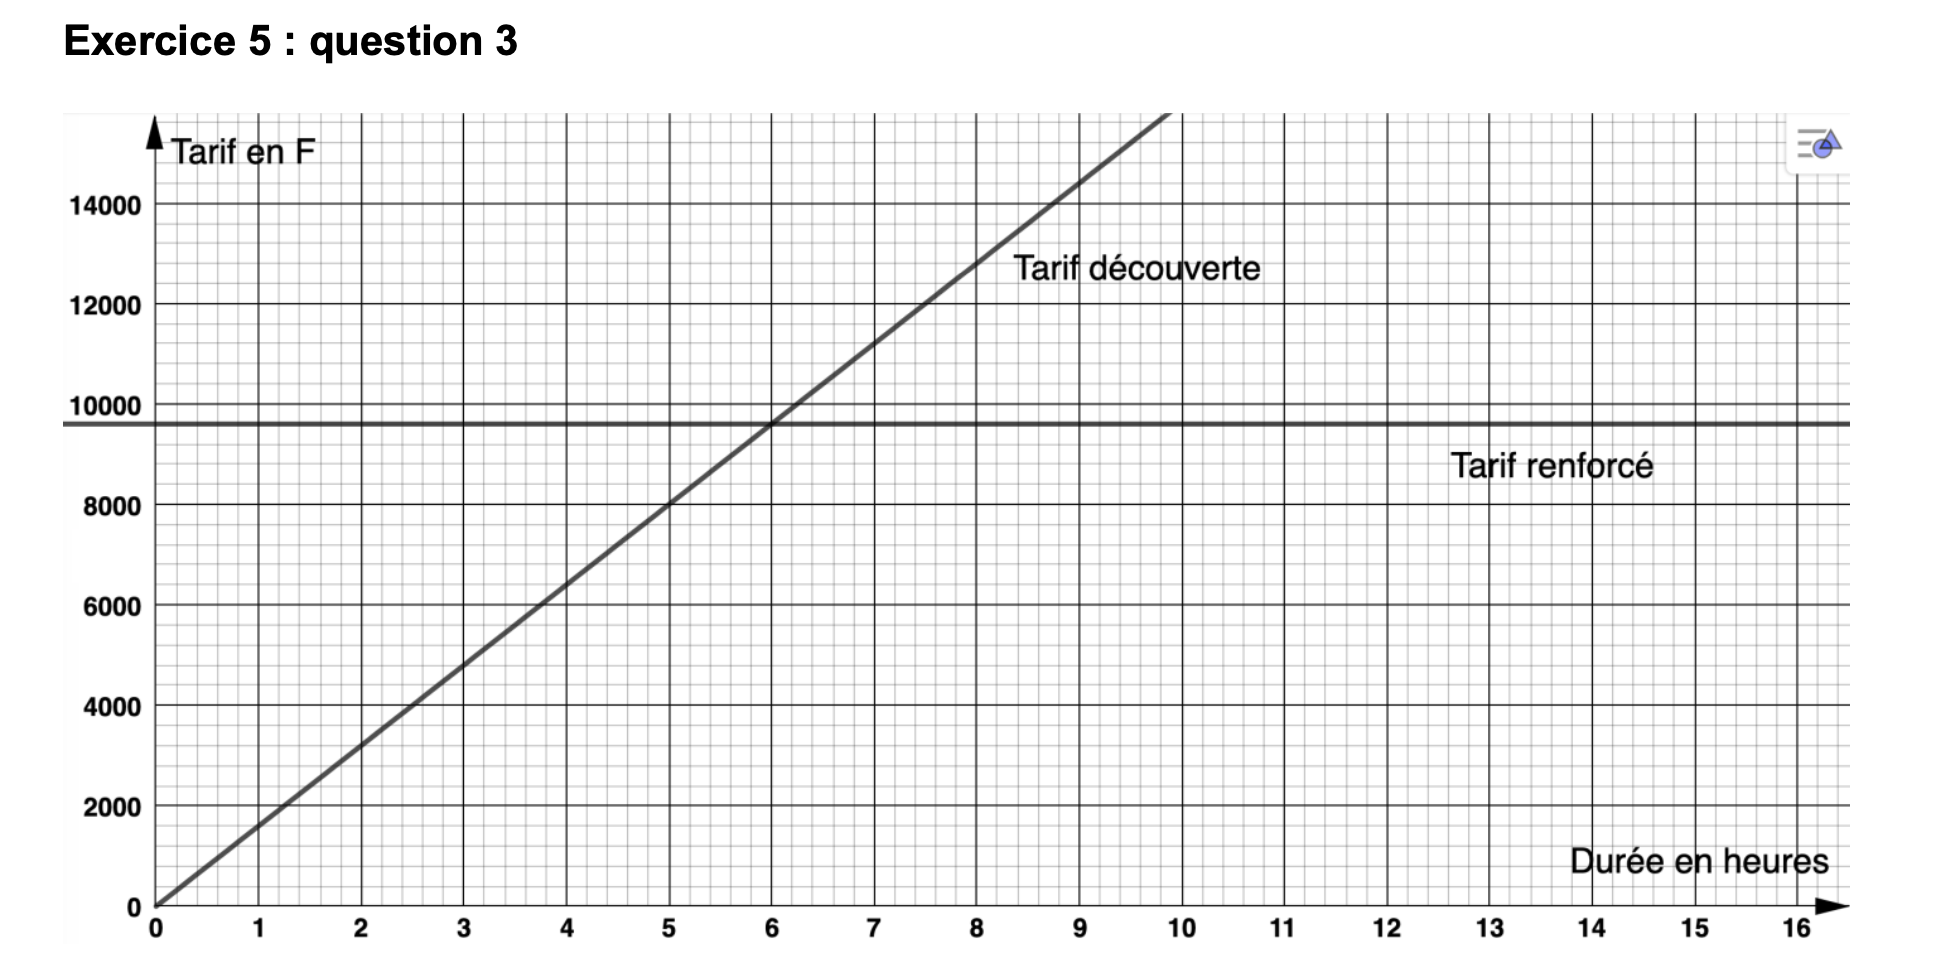
\includegraphics[width = 20 cm]{Ex7A}


\subsection*{Exercice 8 - Asie 2022}	


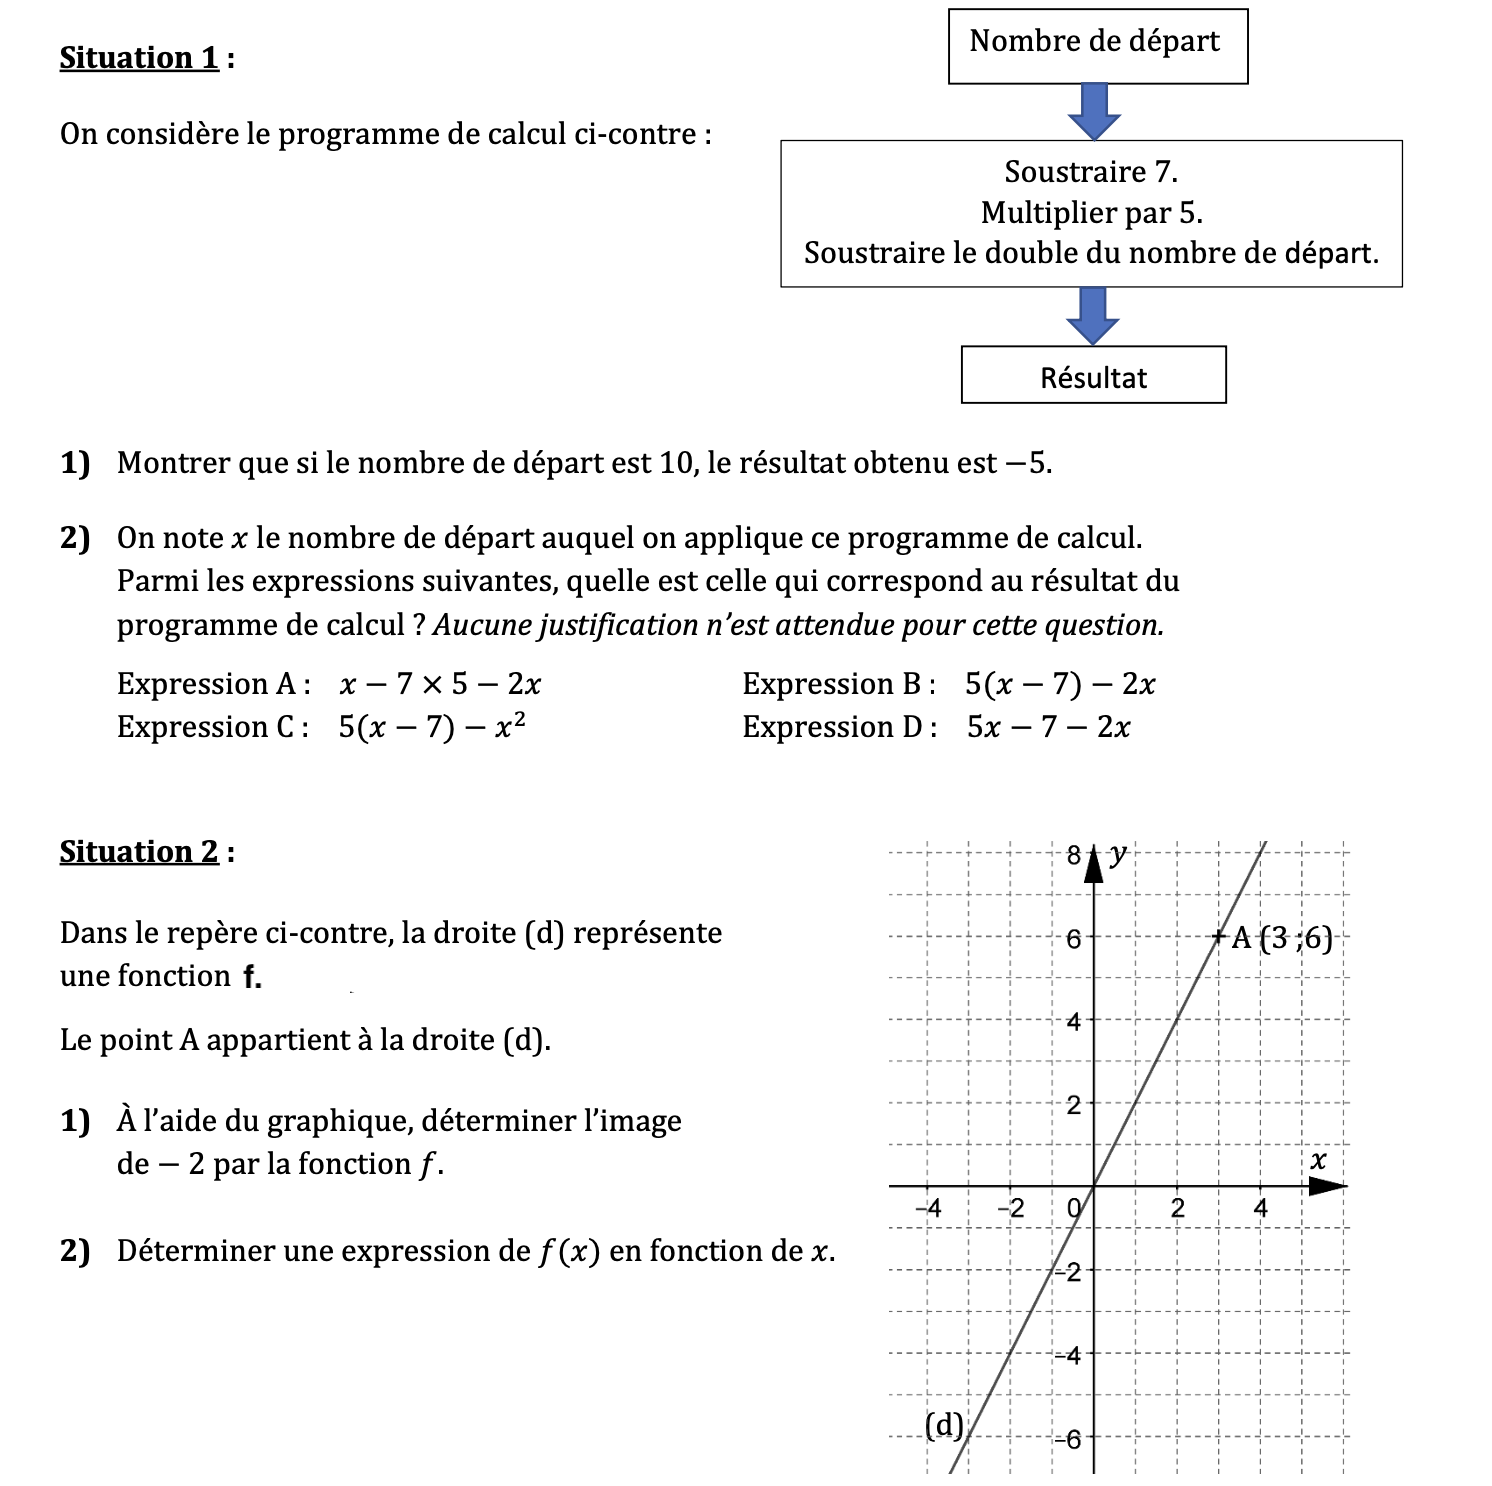
\includegraphics[width = 20 cm]{Ex8}
 	\end{document}
